\subsection{Prototype}


\textbf{Scopo}: Creazionale \\
\textbf{Raggio d'azione}: Oggetti

\paragraph{Definizione} Specifica la tipologia di oggetti da creare utilizzando un'istanza prototipo e creare nuovi oggetti clonando questo prototipo.

\paragraph{Problema} Si pensi ad applicazione che consenta rappresentare degli elementi grafici nel piano cartesiano. L’applicazione potrebbe avere una barra di tasti per effettuare varie operazioni. Un’azione tipica è quella di creare un nuovo oggetto grafico. Per inserire differenti oggetti l’azione da compiere e` identica a parte il tipo di oggetto da creare.

\paragraph{Soluzione} Una soluzione consiste nel configurare l’oggetto responsabile della creazione (il tasto) con un prototipo dell’oggetto da creare.

\begin{figure}[H]
    \centering
    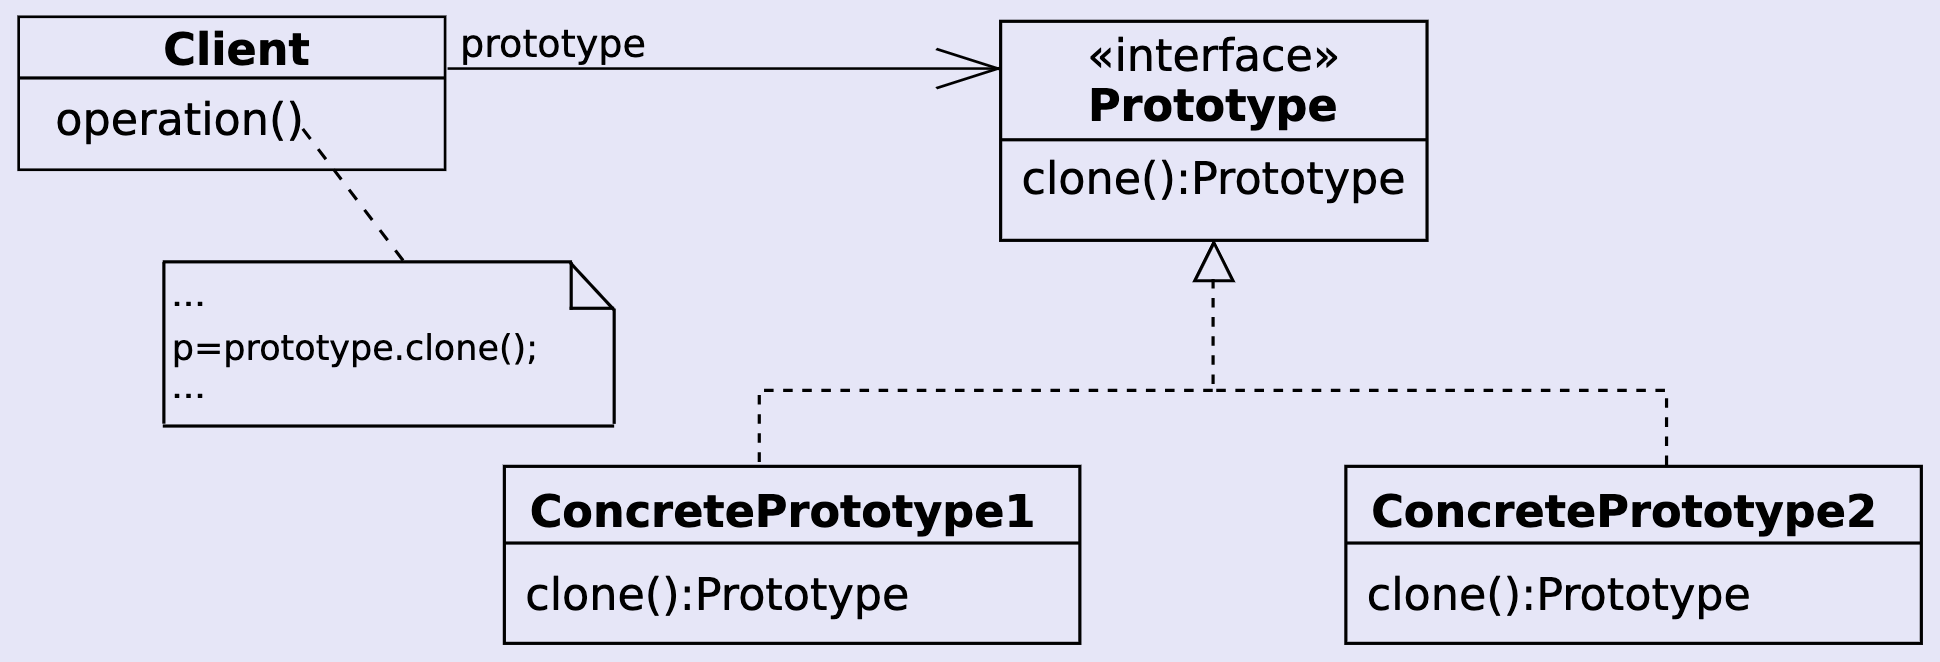
\includegraphics[width=0.75\linewidth]{assets/pattern/prototype/prototype-struttura.png}
    \caption{Struttura del pattern}
\end{figure}

\paragraph{Struttura e Conseguenze} Il pattern è composto da:
\begin{itemize}
    \item \textbf{Prototype}: specifica l'interfaccia che consente la clonazione
    \item \textbf{ConcretePrototype}: implementa l'operazione di clonazione
    \item \textbf{Client}: crea un nuovo oggetto chiedendo ad un prototipo di clonarsi
\end{itemize}

Condivide molte delle conseguenze di Abstract Factory (\ref{abstract-factory}) e Builder (\ref{builder}): nasconde le classi dei prodotti concreti, riducendo il numero di classi che devono essere note al client. In più:
\begin{itemize}
    \item Consente di aggiungere e rimuovere prodotti durante l’esecuzione;
    \item Consente la specifica di nuovi oggetti variando i valori;
    \item Consente la specifica di nuovi oggetti variando la struttura;
    \item Riduce il numero di sottoclassi
    \item Obbliga l'implementazione dell’operazione \textit{clone()}
\end{itemize}

\textbf{In Java}
Utilizzo dell'interfaccia \textit{Cloneable}, è possibile clonare oggetti in modo superficiale (shallow copy) o in maniera profonda (deep copy) ridefinendo il metodo clone().

\begin{minted}[
    fontsize=\footnotesize,
    linenos,
]{java}
// Shallow copy
public class Point2D implements Cloneable {
    private double x; 
    private double y;
    
    @Override public Point2D clone() { 
        try { 
            Point2D clone = (Point2D) super.clone(); 
            return clone;
        } catch (CloneNotSupportedException e) {
            throw new Error(e);
        } 
    } 
}
\end{minted}

\newpage

\begin{minted}[
    fontsize=\footnotesize,
    linenos,
]{java}

// Deep copy
public abstract class PolinomioAstratto implements Polinomio, Cloneable { 
    protected abstract PolinomioAstratto getPrototype(); 

    @Override public Polinomio add(Polinomio p) { 
        // crea un nuovo polinomio 
        Polinomio somma = getPrototype().clone(); 

        // aggiunge ciascun monomio di this al polinomio somma 
        for (Monomio m : this) somma.add(m); 
        
        // aggiunge ciascun monomio di p al polinomio somma 
        for (Monomio m : p) somma.add(m); 
        
        return somma; 
    } 
    
    @Override public PolinomioAstratto clone() { 
        try { 
            return (PolinomioAstratto) super.clone(); 
        } catch (CloneNotSupportedException e) { 
            throw new Error(e); 
        }
    }
}

public class PolinomioLL extends PolinomioAstratto { 
    private static PolinomioLL prototype; 
    private LinkedList<Monomio> monomi = new LinkedList<>(); 
    
    @Override protected synchronized PolinomioLL getPrototype() { 
        if ( prototype==null ) prototype = new PolinomioLL(); 
        return prototype;
    } 
    
    @Override public PolinomioLL clone() {
        PolinomioLL p = (PolinomioLL) super.clone();
        p.monomi = new LinkedList<Monomio>(); 
        for (Monomio m : this) p.monomi.add(m); 
        return p;
    }
}

\end{minted}

\newpage